\subsection{Esercizio 18}
Costruire una function, $hermite.m$, avente una sintassi \underline{analoga} alla function
$spline$ di Matlab (in pratica, con un parametro di ingresso in pi`u per i valori delle derivate),
che implementi, in modo vettoriale, il polinomio interpolante di Hermite.
\newline \textbf{Soluzione:} \newline
% 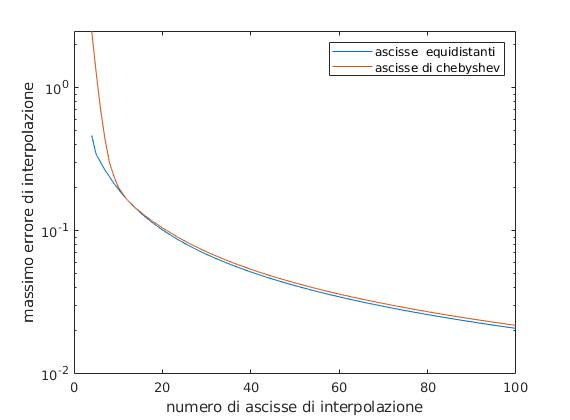
\includegraphics[scale=0.65]{./capitolo4/es18.jpg}